% !TeX spellcheck = de_DE
\chapter{Theoretische Grundlagen}
\label{sec:theorie}
Als schon im Abschnitt "Einleitung" erwähnt wurde, bei der Aufgabestellung es um eine Entwicklung einer Webanwendung geht. Die zu realisierende Software basiert sich, wie die meisten Webanwendungen, auf einer Client-Server-Architektur, wobei der Client Informationen eingibt, während der Server die eingegebene Daten empfängt, bearbeitet und speichert. Eine Webanwendung ist ein Computerprogramm, das eine bestimmte Funktion unter Verwendung eines Webbrowsers als Client ausführt. Die Webanwendung kann so einfach wie ein Kontaktformular auf einer Website oder so komplex wie eine Textverarbeitungs- oder Bildbearbeitungsprogramm sein, die Sie auf Ihr Computer im Browser ausführen können. Um die Webanwendung zu starten, muss der Benutzer keine zusätzlichen Programme installieren. Sie wird auf jedem Gerät mit Browser und Internetzugang ausgeführt. Der Client ist nicht vom Betriebssystem auf dem Computer des Benutzers abhängig. Bei der Entwicklung von Webanwendungen müssen daher keine separaten Versionen für Windows, Linux, Mac OS und andere Betriebssysteme geschrieben werden. Zur Implementierung der Clientseite werden HTML, CSS, JavaScript und Ajax verwendet. Zum Erstellen der Serverseite von Webanwendungen werden Programmiersprachen wie PHP, ASP, ASP.NET, Perl, C / C ++, Java, Python, Ruby und NodeJS verwendet. In dem vorherigen Schritt wurde es die Entscheidung getroffen, die Serverseite mit Web-Framework Django zu erstellen. Django wird mit einem leichten Webserver geliefert, mit dem eine  Website schnell zum Laufen gebracht werden kann, ohne Zeit mit der Einrichtung eines Servers verschwenden zu müssen. Wenn der Entwicklungsserver von Django gestartet wird, überwacht er die Codeänderungen in Echtzeit. Es wird nach dem Ändern des Codes automatisch neu geladen.

In der zu realisierenden Abschlussarbeit ist auch notwendig einen dritten Teil namens Register-Client zu entwickeln, an dem ein RFID-Leser angeschlossen wird. Der Register-Client verfügt selbst über keinen Datenbank und darf nur die abgelesene Daten dem Server schicken. Es geht um eine Simplex-Verbindung, da ein Nachrichtenverkehr asymmetrisch ist, weil der Register-Client keine Daten vom Server zurückbekommen darf und über den erfolgreiche oder gescheiterte Leihvorgang nicht wissen muss. Für die Implementierung des Register-Clients wird uComputer Raspberry Pi benutzt, der möglicherweise nicht der einzige Single-Board-Computer (SBC) auf dem Markt ist, aber bei weitem der beliebteste und schon zur Verfügung im PSE-Labor steht und ergänzend nicht geliefert werden muss. Der Raspberry Pi wird von einer großen Anzahl von Menschen verwendet und viele offizielle und inoffizielle Ressourcen und Produkte umfasst - von Büchern und Zubehör bis zu Schulungen. Dank der Raspberry Pi Foundation werden regelmäßig neue SBC-Modelle veröffentlicht. Der Raspberry Pi eignet sich aufgrund seiner hohen Rechenleistung gut als Desktop-Computer und völlig für die Verwendung in oben geschrieben Zwecken passt . 

\section{Grundlagen der Webanwendungen}
\label{sec:theorie:webapp}
In diesem Kapitel werden die grundlegenden Begriffe zum Entwerfen und Erstellen eines Webanwendung erläutert. Hierbei liegt unser Fokus nicht auf den grafischen Aspekten der Browserfunktionalität (d. H. Dem Layout von Seiten, dem Rendern von Bildern). Stattdessen konzentrieren wir uns auf die Probleme im Zusammenhang mit der Verarbeitung von HTTP-Anfragen und -Antworten. Webanwendungen können abhängig von den verschiedenen Kombinationen ihrer Hauptkomponenten in verschiedene Bestandteilen unterteilt werden. Erstens wird Das Backend (Backend oder Serverteil der Anwendung) auf einem Remotecomputer ausgeführt, der von dem Endnutzer weit entfernt werden kann oder im anliegenden Raum stehen kann.  Es ist in verschiedenen Programmiersprachen zu schrieben. Die Abschlussarbeit wird auf Python Sprache programmiert. Zweitens ist Das Frontend (Frontend oder Client-Teil der Anwendung) im Browser des Benutzers auszuführen. Die Webanwendung könnte theoretisch nur aus dem Client-Teil bestehen, wenn Benutzerdaten nicht länger als eine Sitzung gespeichert werden müssen. Dies aber ist nicht der Fall der Abschlussarbeit, da die Studentenkarten und der Verlauf des Verleihablaufs mindestens für ein laufenden Semester gespeichert werden muss, damit die Mitarbeiter des PSE-Labor immer eine Zugang zu allen gespeicherten vorherigen Leihvorgangs von der Ausleihe bis zur Rückgabe eines Boards. Es ist vorgesehen, dass am Ende des Semester nach dem letzte Rückgabe eines Boards die Datensätzen des zu Ende gegangen Semesters gelöscht wird. 

Da in den letzten Jahren sich Webanwendungen rasant weiterentwickelt und die Desktop-Lösungen schrittweise ersetzt haben und sind zu einem wesentlichen Bestandteil des Geschäfts in der modernen Welt geworden haben, es sollte auch nicht unerwähnt bleiben, welche Vorteile die Webanwendungen haben:
\begin{itemize}
	\item \textbf{Zugriff von jedem Gerät} Die Webanwendung kann überall auf der Welt von einem Computer, Tablet oder Smartphone zugegriffen und verwendet werden. Notwendig ist, dass dem Gerät eine Internetverbindung zur Verfügung steht.

\item \textbf{die Kostenersparnis} Webanwendungen können auf allen Plattformen ausgeführt werden und müssen nicht mehr separat für Android und iOS entwickelt werden.

\item \textbf{Anpassungsfähigkeit} Wenn native Anwendungen bestimmte Betriebssysteme erfordern, jedoch können jedes Betriebssystem (Windows, MAC, Linux usw.) und jeder Browser (Internet Explorer, Opera, FireFox, Google Chrome usw.) für die Arbeit mit einer Webanwendung. ) verwendet werden.

\item \textbf{Keine Software zum Herunterladen} Es ist günstig und einfach dem Endnutzer zu liefern, zu warten und zu aktualisieren. Das Aktualisieren auf die neueste Version erfolgt beim nächsten Laden der Webseite.

\item \textbf{Netzwerksicherheit} Das Websystem verfügt über einen einzigen Einstiegspunkt, der zentral geschützt und konfiguriert werden kann.

\item \textbf{Skalierbarkeit} Mit zunehmender Belastung des Systems ist es nicht erforderlich, die Leistung des Computer von Endbenutzer zu erhöhen. Mit einer Webanwendung kann in der Regel nur mithilfe von Hardwareressourcen eine größere Datenmenge verarbeitet werden, ohne den Quellcode neu zu schreiben und die Architektur ändern zu müssen.

\item \textbf{Verhinderung von Datenverlust} Benutzerdaten werden in der "Cloud" gespeichert, für deren Integrität die Hosting-Anbieter verantwortlich sind, deswegen vom Verlust geschützt, falls die Festplatte des Computers beschädigt wird.
\end{itemize}

Als nächstes geht die Frage nach, wie Client und Server miteinander kommunizieren können. Der Client spricht mit dem Server über \hyperref[sec:appendix:http]{das HTTP-Protokoll}. Das HTTP-Protokoll setzt die Verwendung einer Client-Server-Datenübertragungsstruktur voraus. Die Clientanwendung generiert eine Anforderung und sendet sie an den Server. Anschließend verarbeitet die Serversoftware diese Anforderung, generiert eine Antwort und sendet sie an den Client zurück. Die Clientanwendung kann dann weiterhin andere Anforderungen senden, die auf ähnliche Weise behandelt werden. Wenn ein Webserver eine Anforderung zum Bereitstellen einer statischen Webseite erhält, sendet er die Seite direkt an den Browser.\cite{website:2} Wenn jedoch eine dynamische Seite angefordert wird, sind die Handlungsweise des Webservers nicht so einfach. Der Server übergibt die Seite an ein spezielles Programm, das die letzte Seite bildet. Ein solches Programm wird als Anwendungsserver bezeichnet. Der Anwendungsserver liest den Code auf der Seite, rendert die letzte Seite gemäß dem gelesenen Code und entfernt sie dann von der Seite. Als Ergebnis all dieser Operationen wird eine statische Seite erhalten, die an den Webserver übertragen wird, der sie wiederum an den Client-Browser sendet. Alle Seiten, die der Browser empfängt, enthalten nur HTML-Code.\cite{website:2} Schematische Darstellung des Prozesses kann man auf der Abbildung \ref{fig:client-server}\cite{website:2} ansehen. Die Anforderung kann mit den GET-Methoden erfolgen, wenn wir Daten empfangen möchten, und mit POST, wenn wir die Daten ändern möchten. Die Anfrage enthält auch den Host (Site-Domain), den Anfragetext (wenn es sich um eine POST-Anfrage handelt) und viele zusätzliche technische Informationen. 
\begin{wrapfigure}{l}{0.55\textwidth}
	\fbox{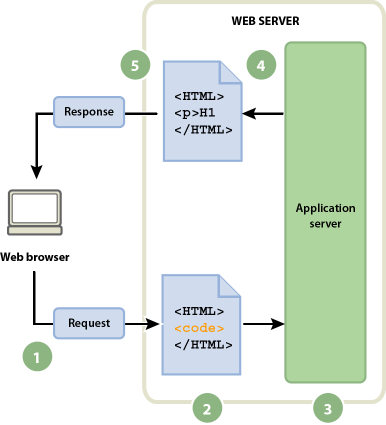
\includegraphics[width=0.52\textwidth]{gfx/ds_process_dynamic.png}}
	\caption{Schematische Darstellung der Client-Server Kommunikation}
	\label{fig:client-server}
\end{wrapfigure}
 Das HTTP-Protokoll ist ein zustandsloses Protokoll auf Anwendungsebene und bietet keine Speicherung von Informationen über die Sitzung des Benutzers; jede Datenübertragung wird als neue Sitzung betrachtet. Da HTTP per Definition ein zustandsloses Protokoll ist, wurde es nicht für die Unterstützung dauerhafter Verbindungen entwickelt. Eine Verbindung sollte lange genug dauern, damit ein Browser eine Anfrage senden und eine Antwort erhalten kann. Eine Verlängerung der Lebensdauer einer Anfrage darüber hinaus wurde nicht unterstützt.\cite[p.62]{shklar:webapplication} 

Am Rande sei auch eine weitere Technologie erwähnt, die uns ständig begegnet. Cache (Cache) ist ein Konzept in der Entwicklung, bei dem häufig verwendete Daten, anstatt jedes Mal aus der Datenbank abgerufen, berechnet oder auf andere Weise vorbereitet, an einem schnell zugänglichen Ort gespeichert werden. Einige Beispiele für die Verwendung des Caches:
\begin{itemize}
	\item Django erhielt eine Anfrage, Daten für ein Diagramm in einem Bericht abzurufen. Daten aus der Datenbank werden abgeholt, vorbereitet und abgelegt in einer Datenbank mit schnellem Zugriff z.B. "memcached", die beispielsweise für eine Stunde zwischengespeichert wird. Bei der nächsten Anfrage werden die notwendigen Daten sofort von "memcached" erhalten und an das Frontend gesendet. Wenn es festgestellt wird, dass die Daten nicht mehr relevant sind, werden sie ungültig beziehungsweise gelöscht aus dem Cache.

	\item CDN-Anbieter (Content Delivery Network) werden zum Zwischenspeichern statischer Dateien verwendet. Hierbei handelt es sich um Servers auf der ganzen Welt, die für die Bereitstellung statischer Inhalte optimiert sind. Manchmal ist es effizienter, Bilder, Videos und JS-Skripte auf einem CDN anstatt auf Ihrem eigenen Server abzulegen.

	\item In allen Browsern ist das statische Zwischenspeichern von Dateien standardmäßig aktiviert. Da die Website nicht zum ersten Mal geöffnet wird, werden die dazugehörige Daten aus dem Zwischenspeichern viel schneller geladen. Der Nachteil für den Entwickler ist, dass bei aktiviertem Cache die vorgenommenen Änderungen nicht immer sofort sichtbar sind. 
\end{itemize}

Daraus lässt sich die Schlussfolgerung ziehen, dass eine Webanwendung für einen Endnutzer wie eine Website aussieht, auf der  die Webseiten mit teilweise oder vollständig nicht formatiertem Inhalt sich befinden. Die Endfertigung des Inhalts findet nur dann statt, nachdem ein Website-Besucher die Seite vom Webserver angefordert hat. 

In diesem Kapitel wurden die Grundlagen der Webanwendungen und des HTTP-Protokolls erörtert. Diese Diskussion war nicht als umfassende Beschreibung aller Funktionen gedacht, eher als Überblick über das Verständnis und die Arbeit mit aktuellen Stand der Technologie und zukünftigen Verwendung der entwickelte Software im PSE-Labor. 

\section{Raspberry Pi Board und Betriebsystem }
\label{sec:theorie:raspberry}
\begin{wrapfigure}{l}{0.45\textwidth}
	\fbox{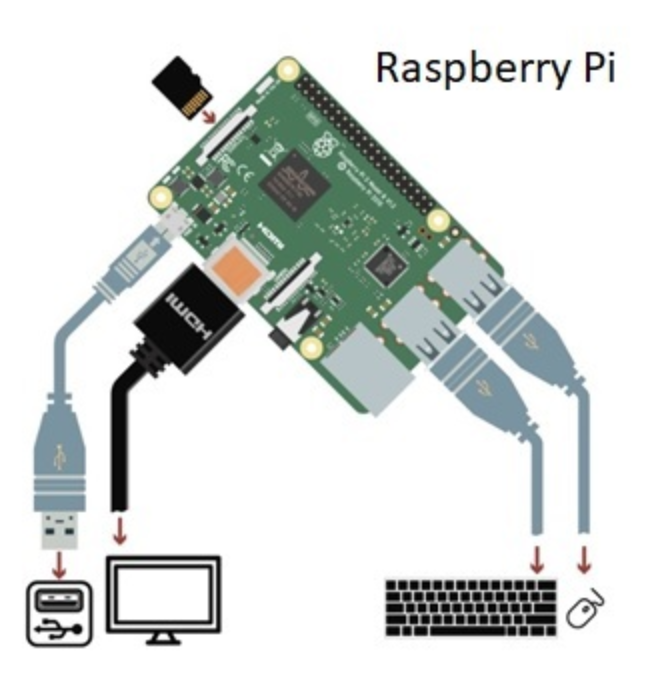
\includegraphics[width=0.42\textwidth]{gfx/rasp.png}}
	\caption{Peripherieanschlüsse des Mikrocomputers}
	\label{fig:rasp}
\end{wrapfigure}
Raspberry Pi ist ein Einplatinencomputer, wobei die verschiedene Teile des Computers, die sich normalerweise auf separaten Platinen befinden, werden hier nur auf einer dargestellt. Wie die meisten Einplatinencomputer ist der Raspberry Pi so klein wie eine Kreditkarte. Jedoch bedeutet das nicht, dass er nicht leistungsstark ist: Ein Raspberry Pi kann alles, was ein größerer und leistungsfähiger Computer kann, aber nicht unbedingt gleich schnell. Der Produktname kombiniert Raspberry-Himbeer- und Pi- die Kraiszahl Pi. Das Himbeerbild wurde zum Logo des Projekts. Der Raspberry Pi ist eine kostengünstige Plattform - sein empfohlener Verkaufspreis beträgt weniger als 50€. Ein Mikrocomputer verfügt über alle Funktionen eines Personal Computer (PC): Prozessor, Speicher, Betriebssystem, Anschluss an einen Monitor (TV), die Vernetzung. Der Raspberry Pi verfügt im Gegensatz zu einem PC über zusätzliche Peripheriegeräte wie GPIO-Ports (General Purpose Input / Output). Über diese Pins kann der Mikrocomputer mit der elektronischen Welt der Sensoren, Bildschirmen und Aktoren interagieren. In Abbildung \ref{fig:rasp}\cite{website:3} sind die Anschlüsse schematisch dargestellt.

\begin{wrapfigure}{l}{0.45\textwidth}
	\fbox{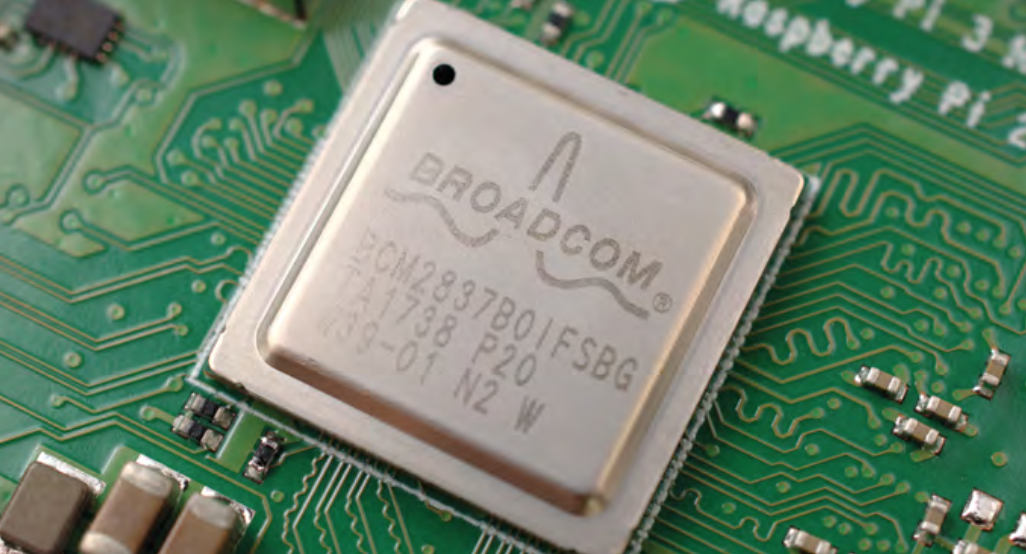
\includegraphics[width=0.42\textwidth]{gfx/system-on-chip.png}}
	\caption{The Raspberry Pi’s system-on-chip (SoC)}
	\label{fig:rasp_soc}
\end{wrapfigure}

Für die Entwicklung der Abschlussarbeit und die Verwendung im Labor wird Raspberry Pi 3 Model B+ benutzt, an dem der RFID Leser angeschlossen wird. Das Modell "Raspberry Pi 3 B" ist eine kontinuierliche Weiterentwicklung zum Vorgängermodell "Raspberry Pi 2 B".
Der Raspberry Pi 3 enthält einen Quad-Core-Prozessor mit 1,2 GHz von Broadcom und einen SDRAM-Arbeitsspeicher mit 1 GByte. Wie jeder Computer besteht der Raspberry Pi aus verschiedenen Komponenten, von denen jede eine Rolle in der Zusammenarbeit spielt. Die erste und wohl wichtigste davon befindet sich direkt über dem Mittelpunkt auf der Oberseite der Platine (Abbildung 1-2) und ist mit einer Metallkappe bedeckt: dem System-on-Chip (SoC). Der Name System-on-Chip ist ein guter Indikator dafür, was wird gefunden, wenn die Metallabdeckung abgenommen wird: einen Siliziumchip, der eine integrierte Schaltung ist und den Großteil des Raspberry Pi-Systems enthält. Dazu gehören die Zentraleinheit (CPU), die gemeinhin als „Gehirn“ eines Computers bezeichnet wird, und die Grafikverarbeitungseinheit (GPU), die die visuelle Seite der Dinge übernimmt.\cite[p. 11]{gareth:raspi} Auf der Unterseite des Raspberry Pi befindet sich einen weiteren Chip, der wie ein kleines schwarzes Plastikquadrat aussieht. Dies ist der Direktzugriffsspeicher (RAM) des Mikrocomputers. Wenn am Pi gearbeitet wird, wird die laufende Arbeit auf dem RAM gespeichert. Nur wenn die Daten explizit auf die microSD-Karte geschrieben werden, dann werden sie zum nächsten Verwendung gespeichert und nach dem Ausschalten nicht gelöscht. Zusammen bilden diese Komponenten die flüchtigen und nichtflüchtigen Speicher des Pi: Der flüchtige RAM verliert seinen Inhalt, wenn der Pi ausgeschaltet wird, während die nichtflüchtige microSD-Karte seinen Inhalt behält. Der Raspberry Pi  nicht den Austausch des aktuellen RAM-Chips. Der aktuelle RAM-Chip ist als BGA-Gehäuse direkt auf die Oberseite der CPU gelötet, was das Entfernen und / oder Ersetzen sehr schwierig macht, selbst wenn Sie den kompatiblen größeren Speicherchip finden könnten. Die Aufbau des Pi Der unterstützt den Austausch des aktuellen RAM-Chips nicht. Der aktuelle RAM-Chip ist als BGA-Gehäuse direkt auf die Oberseite der CPU gelötet. Das Hartlöten macht das Entfernen und / oder Ersetzen des RAMs sehr schwierig und deshalb es ist beim Kauf des bestimmtes Board auf die Große des RAMs zu achten.

Die Besonderheiten des Raspberry Pi 3 ist, dass WLAN nach IEEE 802.11 b/g/n und Bluetooth Low Energy onboard sind und nicht durch externe USB-Adapter nachgerüstet werden müssen. Es ist für die vorgesehene Aufgabe wichtig ist, da die erforderlichen Komponenten nicht zusätzlich gekauft werden muss, was das Budget der PSE-Labors erspart und eine gewisse Zeit nicht geplant muss, dass die zusätzlich gekauften Komponenten irgendwie zum funktionieren bringen. Hier gab es in der Vergangenheit immer wieder Schwierigkeiten mit der Hardware-Erkennung oder Treiber-Probleme. 

Die ARMv8-Architektur enthält Cortex-A53-Rechenkerne, die bei gleichem Takt schneller sind als die alten Cortex-A7-Kerne des Raspberry Pi 2 B. Von der 64-Bit-Fähigkeiten der ARMv8-Architektur profitiert allerdings nur neue Software, da 64 Bit auf der Hardware-Seite allerdings vom Betriebssystem und der Software auch unterstützt werden muss. Die folgende Liste gibt es eine kurzen Ansicht auf die Architektur des Mikrocomputers.
\begin{itemize}
\item System-on-Chip: BCM2837 64 Bit ARMv8 von Broadcom
\item Prozessor: Quad-Core-Prozessor mit 1,2 GHz
\item GPU: Dual-Core-GPU VideoCore IV mit OpenGL ES 2.0 und OpenVG mit Hardwarebeschleunigung und 1080p30 H.264 High-Profile-Decoding
\item Arbeitsspeicher: 1 GByte LPDDR2-SDRAM
\item WLAN: BCM43143 onboard für IEEE 802.11b, g und n im 2,4 GHz-Bereich
\item Bluetooth: Bluetooth Classic und Low Energy (BLE) onboard (Bluetooth 4.1)  
\end{itemize}
Eines der beliebtesten Betriebssysteme für den Raspberry Pi ist das Raspbian-Betriebssystem. Das Raspbian-Betriebssystem Raspbian basiert auf der ARM-Version von Debian 8 Jessie, ist für die Raspberry Pi-Hardware optimiert  und enthält die Standardprogramme wie die LibreOffice Office Suite, einen Webbrowser, Claws Mail, eine leichtgewichtige Desktop-Umgebung und einige Programmier-Lernwerkzeuge. Neuere Versionen des Betriebssystems Raspbian verfügen über einen völlig modernen Chromium-Browser, mit dem auch komplexe Webseiten korrekt angezeigt werden können. Um eine Information auf einem großen Bildschirm anzuzeigen, wird Chromium nur im Vollbildmodus gestartet, den Mauszeiger ausgeblendet und den Bildschirmschoner ausgeschaltet. Es gibt verschiedene Möglichkeiten, Raspbian auf einem Raspberry Pi 3 zu installieren. Die erste besteht darin, das Dienstprogramm NOOBS zu verwenden, die zweite darin, den Inhalt des Bildes des Betriebssystem direkt auf die Karte zu schreiben. Während der Entwicklung des Register-Clients wurde das Betriebssystem auf MicroSD-Karte geschrieben. Das Raspbian-Betriebssystem bootet von einer Micro-SD-Karte und das gesamte Betriebssystem läuft von der Karte. 

Nach der kurzen Beschreibung der Raspberry Pi Architektur und sein Betriebssystem Raspbian ist schlusszufolgern, dass die Verwendung eines Raspberry Pi Mikrocomputers für die Implementierung des Register-Klient mit dem angeschlossenen RFID Leser ist eine lohnenswerte Entscheidung für in dieser Abschlussarbeit geschriebenen Aufgabe.  


\section{Kontaktlose Smartcards MIFARE}
\label{sec:theorie:mifare}
Anfänglich war die Smartcard eine Plastikkarte im ID-1-Format mit einer Größe von 85,60 × 53,98 mm und abgerundeten Ecken (eine Standardbank / Kreditkarte hat die gleiche Form und Abmessungen). Darin ist ein Mikrochip eingebettet, dessen Kommunikationskontakte zu einer Seite herausgeführt werden. Später erschienen Smartcards im ID-000-Format, sie wurden in Mobiltelefonen verwendet und sind uns als SIM-Karten bekannt. Dann erschienen Smartcards ohne externes Kontaktfeld, und sie begannen, einen Funkkanal für die Kommunikation und Energieübertragung zu verwenden. Smartcards haben keine eigene Stromquelle und sind auf eine externe angewiesen. Der Hauptvorteil einer Smartcard ist die physische Sicherheit der darauf gespeicherten Daten. Der Mikrochip ist sehr klein und alles notwendiges befindet sich darauf, ohne dass interne Kontakte hergestellt werden müssen, an die es sich zum Abfangen angeschlossen werden kann. 

Der ungefähre Lebenszyklus einer Smartcard (z. B. einer Bankkarte mit Chip) besteht aus mehreren Phasen. Daran sind der Chiphersteller, der Smartcard-Hersteller, der Kunde und der Kunde beteiligt:

\begin{itemize}
	\item \textbf{Herstellung von Chips/Prozessoren}. Zu diesem Zeitpunkt schreibt der direkte Hersteller des Chips nach der physischen Produktion die vom Hersteller der Smartcards bereitgestellte universelle und für alle Karten des gleichen Typs dieselbe Firmware auf.
\item \textbf{Initialisierung der Smartcard}. Die Chips werden an den Kartenhersteller gesendet. Er ändert die Firmware nach Bedarf. Beispielsweise schreibt er eine eindeutige Seriennummer in jede Karte. Anschließend deaktiviert er die Möglichkeit, diese mit einer speziellen Anforderung zu ändern.
\item \textbf{Smartcard-Herstellung}. Der Hersteller legt den Chip in Karten des gewünschten Formats ein und sendet diese an den Kunden, beispielsweise eine Bank.
\item \textbf{Personalisierung}. Der Kunde schreibt unter Verwendung der Methoden der Firmware auf der Karte seine Anwendungen darauf, z. B. Bankgeschäfte. sowie zusätzliche Daten, z. B. Kundenname, Kontonummer usw. Danach wird die Karte durch eine spezielle Anfrage finalisiert, wonach beispielsweise die Aufzeichnung neuer Anträge eingeschränkt wird.
\item \textbf{Ausgabe}. Die Karte wird dem Kunden ausgegeben und vom Kunden verwendet.
\item \textbf{Zerstörung}. Die Karte wird weggeworfen.
\end{itemize}

\begin{figure}
	\centering
	\fbox{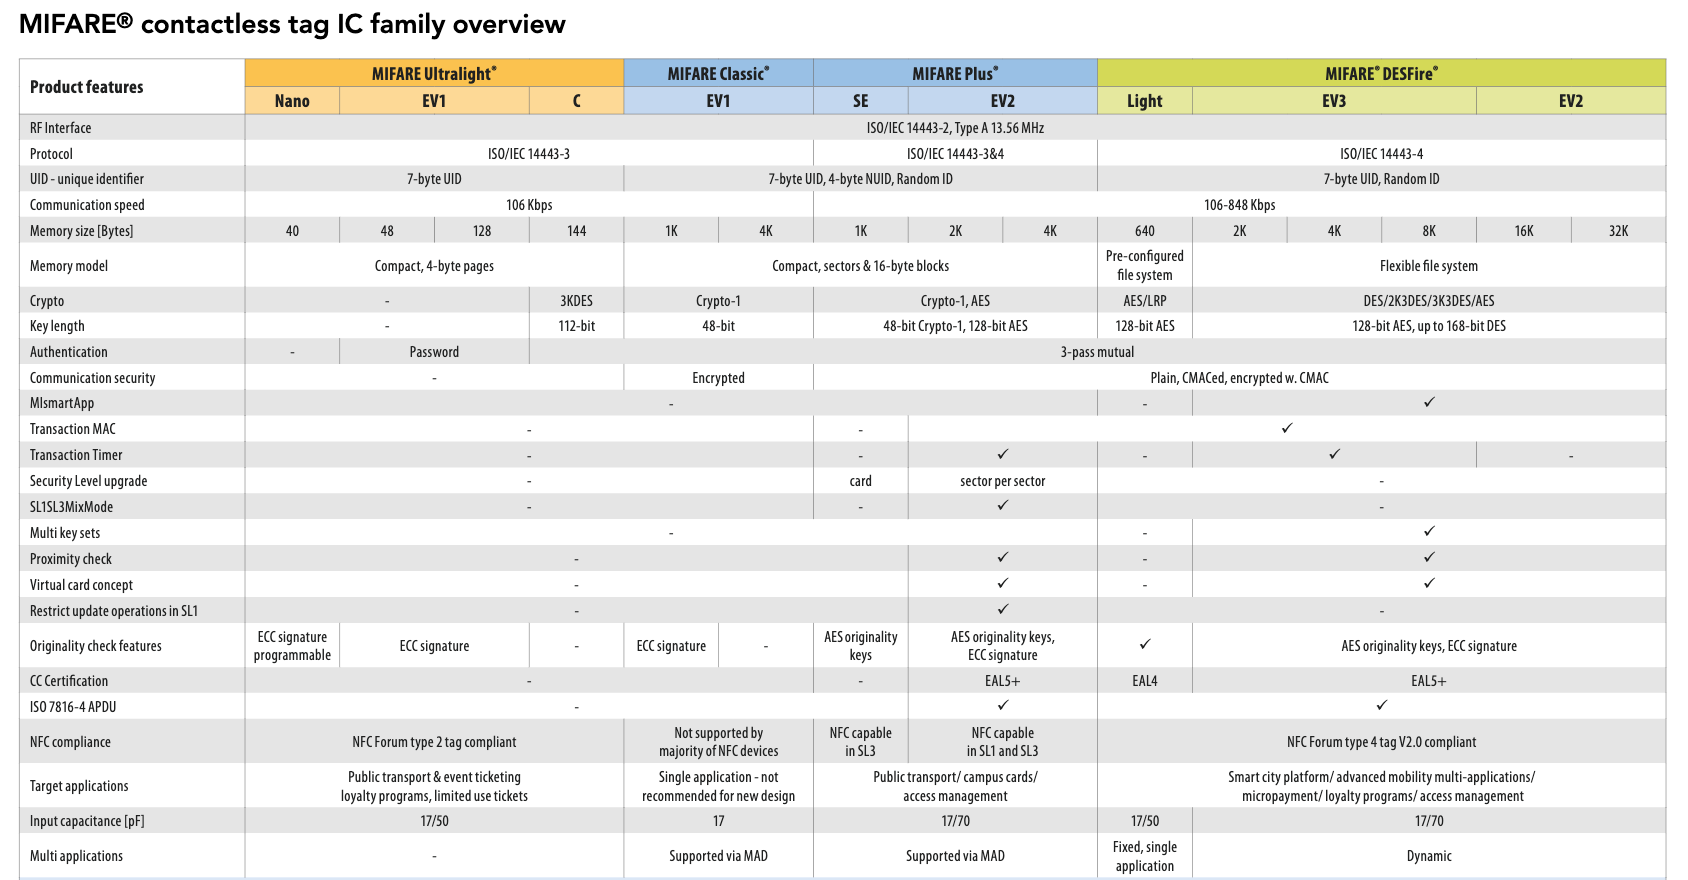
\includegraphics[width=1\textwidth]{gfx/mifare.png}}
	\caption{Mifareproduktfamilie}
	\label{fig:mifare}
\end{figure}


Einer der größten Hersteller von Smartcards ist die Firma NXP Semiconductors mit Hauptsitz in den Niederlanden. Mit einer großen Produktvielfalt schafft diese Lösungen für kontaktlose Zugangs-und Zeitkontrollen und sichere kontaktlose Automobilzugangskontrollen. Die welt-weit meistgenutzte kontaktlose Chipkartentechnik „MIFARE“ wurde von NXP Semiconductors entwickelt und die Produktfamilie umfasst mittlerweile vier Produktreihen.(siehe Abbildung \ref{fig:mifare})\cite{website:9} Alle MIFARE-ICs sind konform zur Norm ISO/IEC 14443 und erfüllen somit die Standards für die kontaktlose Kommunikation zwischen Chipkarten. Sie arbeiten mit 13,56 MHz und ihre Leseentfernung ist bis 10 cm möglich. Kontaktlose MIFARE-Smartcards verfügen über einen 1-KByte-Speicher, der in 16 Sektoren mit jeweils 16 Byte unterteilt ist. Die Datenspeicherdauer beträgt bis zu 10 Jahre. Die Anzahl der Umschreibzyklen beträgt 100.000 Zyklen.

Neben NXP Semiconductors werden Chips für Mifare-Smartcards von der deutschen Firma Infineon im Rahmen einer Lizenzvereinbarung hergestellt\cite{website:11}. Nur Smartcards mit Chips von NXP Semiconductors und Infineon dürfen die Marke Mifare in ihrem Namen tragen. Nur Karten mit diesen Chips können als "Original" bezeichnet werden.

Die Studentenkarte der Beuth Hochschule wurden mit Mifare DESfire EV1 Kartenchip hergestellt. MIFARE DESFire EV1 ist die nächste Generation von Mifare Desfire mit einigen verbesserten Funktionen der Sicherheit und Verschlüsselung\cite[p.83]{chirico:smart_card}. Unberechtigte können sie aufgrund der AES-Verschlüsselung nicht auslesen. Zudem enthalten die Karten elektronisch keine persönlichen Daten\cite{website:12}. Alle auf der Karte gespeicherte Daten werden kodiert, z.B. mit der UID der einzelnen Karte verschlüsselt. MIFARE DESFire wird in vielen NFC- und RFID-Anwendungen verwendet, da er als sicherer Transponder mit einem von drei verschiedenen Typen von Verschlüsselung gesichert ist: Single DES, Triple DES oder AES. Im Allgemeinen wird AES als die sicherste Verschlüsselungsstufe der oben aufgeführten Methoden angesehen. Der AES-Authentifizierungsprozess besteht aus mehreren Schritten, in denen der NFC / RFID-Reader und das MFDFEV1-Tag verschlüsselte Daten austauschen, um zu überprüfen, ob sie denselben Schlüssel verwenden. Während dieses Vorgangs wird ein Sitzungsschlüssel erstellt, der für bestimmte Befehle wie den ChangeKey-Befehl verwendet wird\cite{website:10}.

Zusammenfassend lässt sich sagen, dass die neue Studentenkarte, die an der Beuth Hochschule ab Sommersemester 2018 verwendet wurden, sind eine zuverlässige und zeitgemäße Lösung. Da die Karte elektronisch keine persönlichen Daten der Studierenden beinhaltet und die Automaten alle persönlichen Daten anhand eines Pseudonyms online abrufen müssen (d.h. liegen in den Automaten auch keine persönlichen Daten vor), es in Fall des Verlusts die persönliche Daten von den Unberechtigte nicht ausgelesen werden können\cite{website:12}. Das stand im Fokus der Entscheidung, eine Studentenkarte als einzige elektronischer Identifizierungsmittel beim Ausleihe/Rückgabevorgänge im PSE-Laboz zu benutzen.


\section{Sender-Empfänger-System mit RFID}
\label{sec:theorie:rfid}
Im vorherigen Kapitel \ref{sec:theorie:mifare} wurden die Grundlagen und Vorteilen der MIFARE-Technologie für Smartcards erklärt. Im aktuellen Kapitel wird über die  Sender-Empfänger-System mit RFID beschrieben. Für die Implementierung der Aufgabe wird sowohl MIFARE-Smartcards als auch RFID-Tag-Mikrochips verwendet. Der letzte wird zum Identifizierung der auszuleihenden Raspi-Boards benutzt und auf der Rückseite des jeden Boards unter dem Schutzschirm geklebt werden. Beide Typs können mit dem RFID-Leser ACR122U-A9 von Advanced Card Systems abgelesen werden. Ab hier wird weiter nur den Begriff "Tag" sowohl für MIFARE-Smartcards als auch für RFID-Tag-Mikrochips verwendet und den Unterschied in Namen nicht weiter angemerkt. Die gespeicherte Daten warten darauf, gelesen zu werden. Die Antenne des Tags erhält Energie von einer RFID-Leseantenne. Mit der Stromversorgung der internen Batterie oder des Lesegeräts sendet das Tag Funkwellen an das Lesegerät zurück. Der Leser nimmt die Funkwellen des Tags auf und interpretiert die Frequenzen als Daten. RFID-Tags, die über einen Teil des elektromagnetischen Spektrums gesendet werden, und die genaue Frequenz können ausgewählt werden, um Interferenzen mit anderen elektronischen Geräten zu vermeiden. Der Leser sendet ein Signal an das Tag und liest seine Antwort\cite{website:13}. Der Leser verfügt über einen Funkempfänger, der als Transceiver bezeichnet wird und ein codiertes Funksignal an das Tag sendet. Das Signal aktiviert das Tag und der Transponder wandelt das Signal dann in eine nutzbaren Leistung um und sendet auf den Leser. Das Tag empfängt die Nachricht und antwortet dann mit seiner Identifikation und anderen Daten. Dies kann eine eindeutige Seriennummer des Produkts oder produktbezogene Daten sein. In der Abschlussarbeit wird nach der UID des Tags gefragt. 

\begin{wrapfigure}{l}{0.45\textwidth}
	\fbox{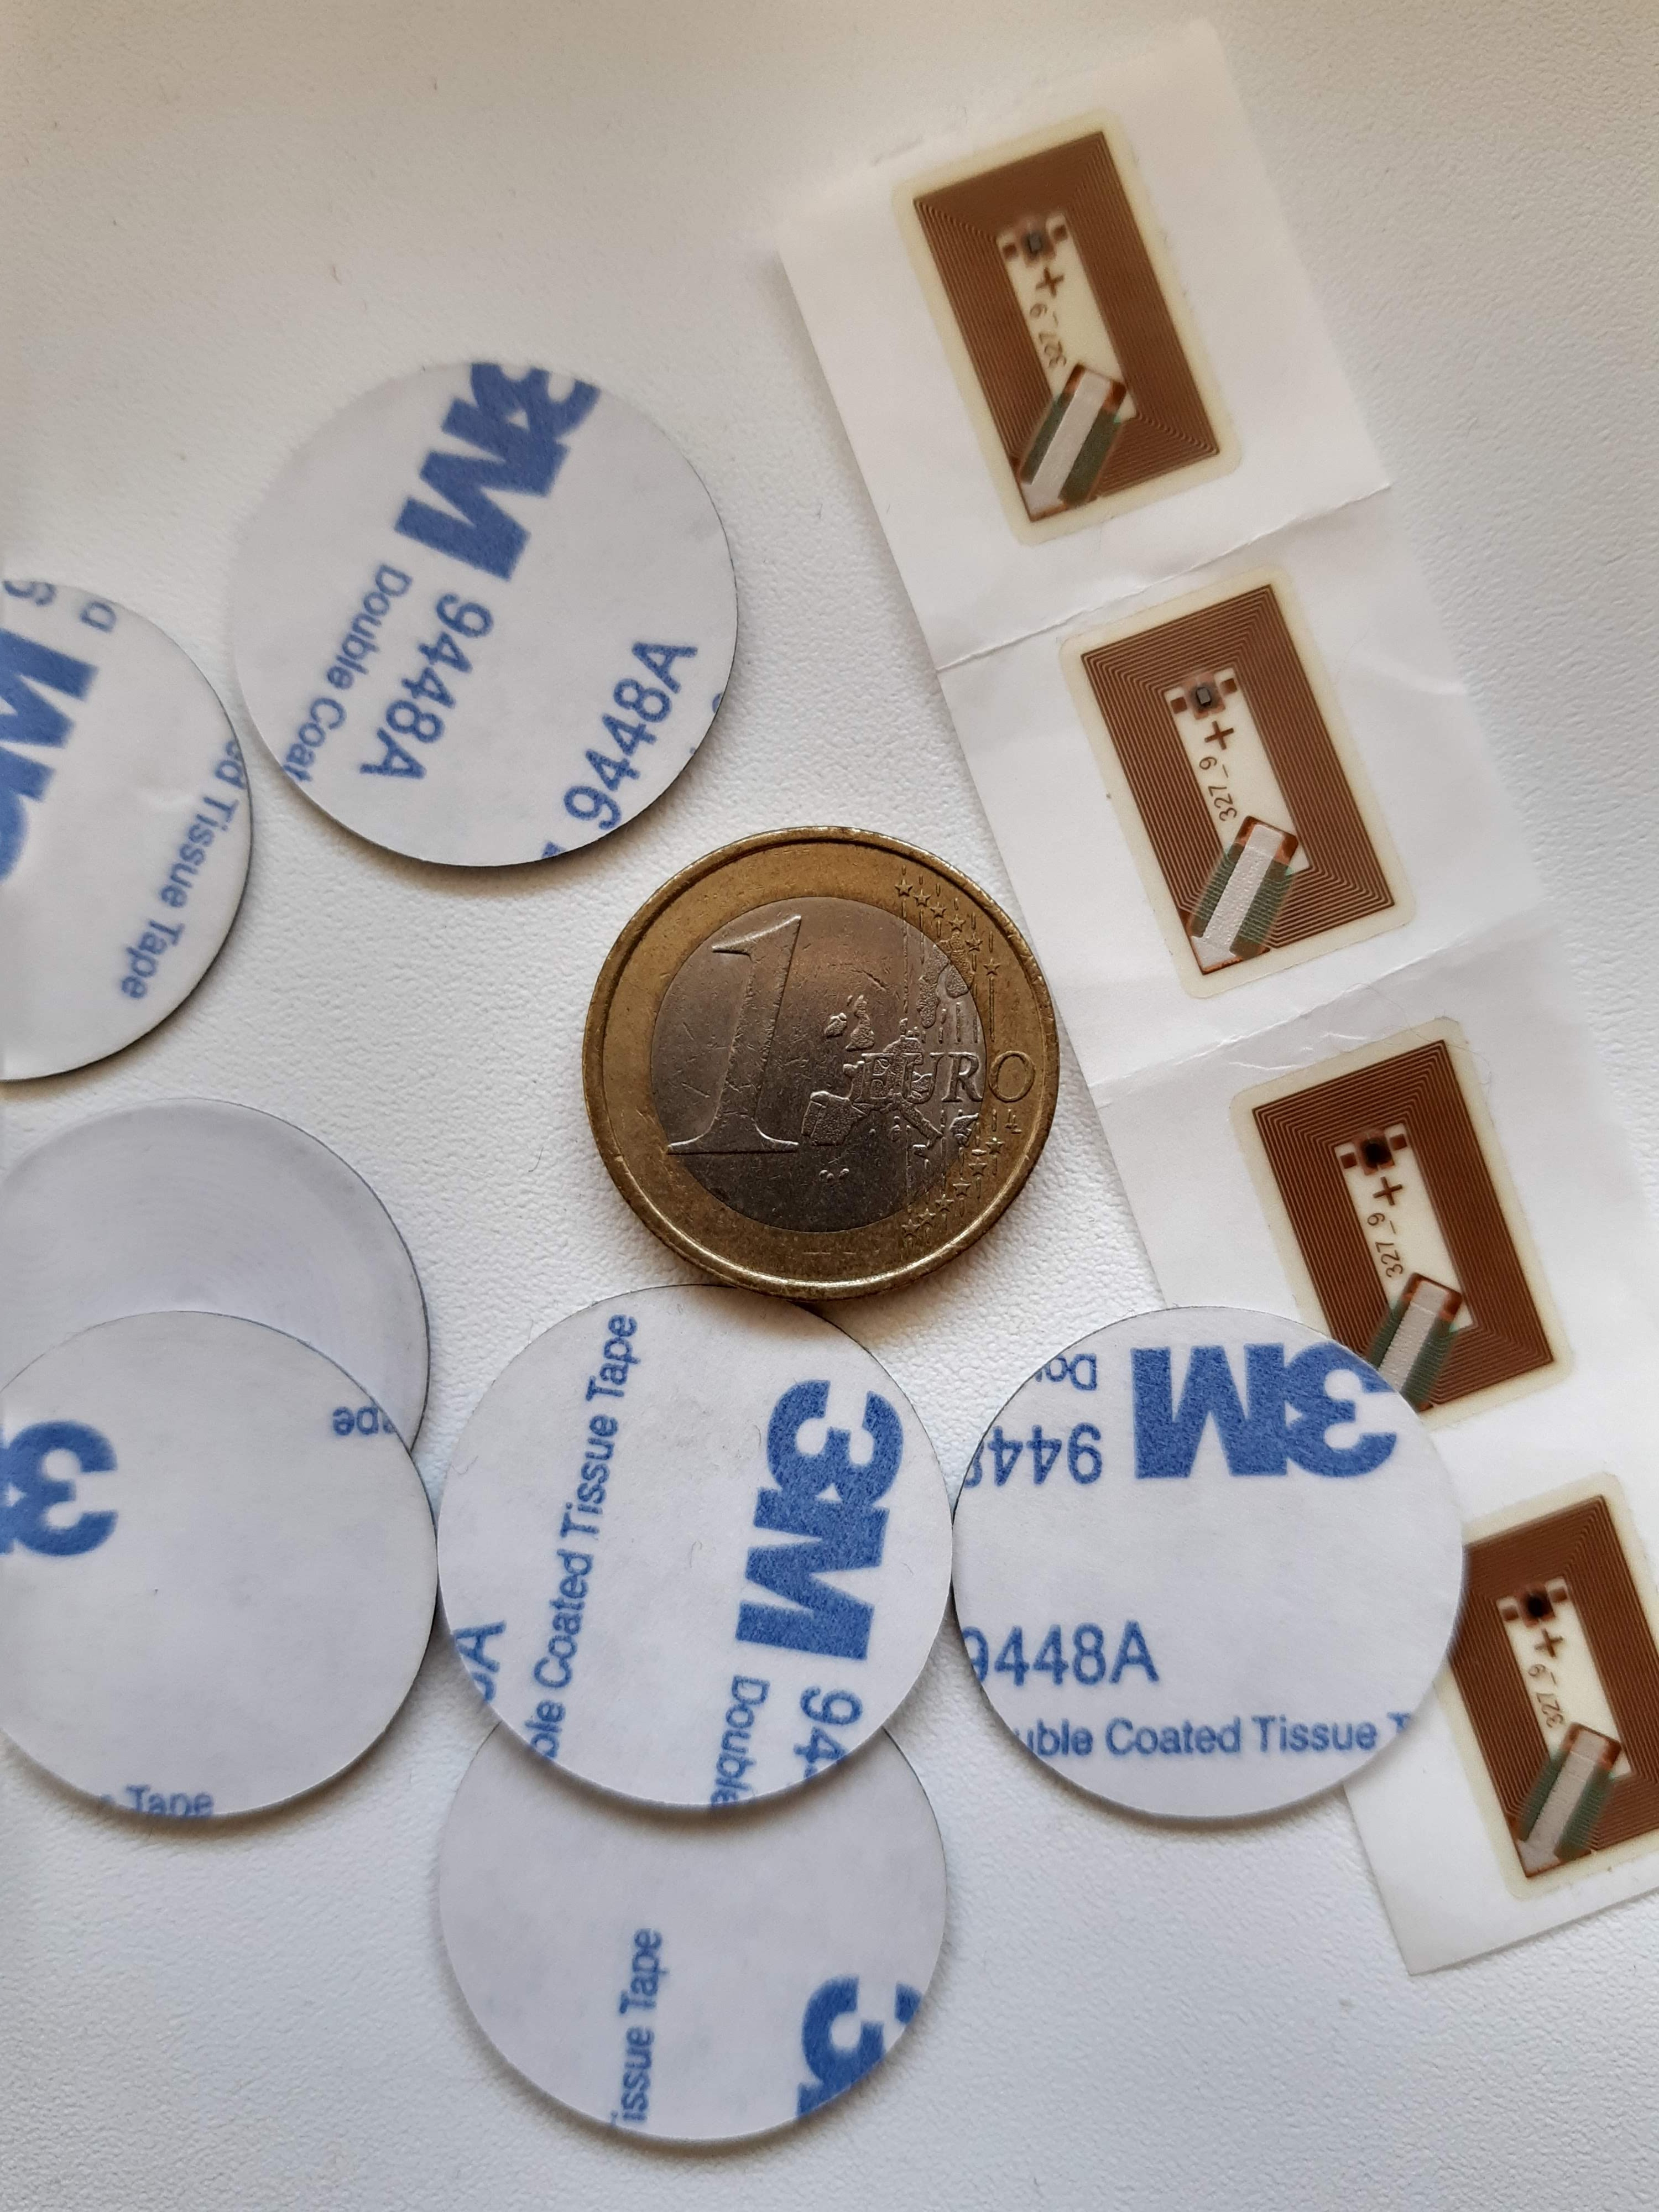
\includegraphics[width=0.42\textwidth]{gfx/tags.jpg}}
	\caption{Verschiedenen RFID-Tags}
	\label{fig:tags}
\end{wrapfigure}
Während sich jedes Sender-Empfänger-System mit RFID hinsichtlich Gerätetyp und Komplexität unterscheidet, enthält jedoch jedes RFID-System mindestens die folgenden vier Komponenten: Leser, Antennen, Tags und Kabel. Das einfachste System kann aus einem mobilen Hand-RFID-Lesegerät (mit integrierter Antenne) und RFID-Tags bestehen, während komplexere Systeme mit Multi-Port-Lesegeräten, GPIO-Boxen, zusätzlichen Funktionsgeräten, mehreren Antennen, Kabeln und RFID-Tags ausgelegt sind und ein komplettes Software-Setup benötigen können. RFID-Tag-Typ Bestimmt das RFID-System. Derzeit gibt es drei verschiedene Arten von Tags: \textbf{aktiv, semi-passiv und passiv}. Ein aktives Tag sendet mit seiner Batterie Radiowellen an einen Leser, während eine semi-passive Tag-Batterie in Gegenwart eines Lesers aktiviert wird. Aktive und semi-passive Tags werden über größere Entfernungen gelesen. Sie senden hohe Frequenzen von 850 bis 950 MHz, die von 30 Meter oder mehr gelesen werden können. Zusätzliche Batterien können die Reichweite eines Tags auf über 90 Meter erhöhen. Passive RFID-Tags haben keine Batterie und verwenden die vom Lesegerät übertragene Funkenergie als Stromquelle. Diese Tags werden bis zu ein paar Meter entfernt gelesen und sind kostengünstiger\cite{website:13}. Für die Markierung der Raspi-Boards im PSE-Labor werden die passive RFID-Tags verwendet, die für vorgesehenen Zwecken ideal dienen. Die runde benutzte im Abschlussprojekt RFID-Tags sind auf der Abbildung \ref{fig:tags} im Vergleich in der Große zu 1-Euro Münze zu sehen. RFID-Systeme können nach Tag- und Lesertyp klassifiziert werden: passiver Leser - aktiver Tag (PRAT), aktiver Leser - passiver Tag (ARPT) und aktiver Leser - aktiver Tag (ARAT). Das ARPT-System wird im PSE-Labor eingesetzt und verfügt über einen aktiven Leser und empfängt Authentifizierungssignalantworten von passiven Tags. Ich möchte an dieser Stelle auch noch anmerken, dass der Initialisierungsprozess für eine kontaktlose Karte viel komplizierter als für eine Kontaktkarte ist. Das meiste davon wird vom sogenannten Antikollisionszyklus besetzt. Eine Kollision tritt auf, wenn mehr als eine Karte gleichzeitig auf das elektromagnetische Feld der RFID-Leser trifft und der diese Karten voneinander unterscheiden muss. Der Algorithmus dieses Prozesses ist sehr komplex und umfasst mehrere zehn Seiten Beschreibung in den Normen ISO/IEC 14443-2 und ISO / IEC 14443-3. Daher werde ich ihn hier nicht angeben, da es nicht von Entwickler wirklich etwas zu machen benötigt wird - das Terminal und der RFID-Leser sind voll damit beschäftigt.

An dieser Stelle muss es gesagt werden, dass die RFID-Tags bestimmte Nachteile haben, die wurden zwischen den Mitarbeiter und Autorin der Abschlussarbeit diskutiert. Es wurde jedoch die Entscheidung getroffen, dass für die vorgesehenen Zwecken des Verfolgen, welchen Raspi-Board von welchem Student am welchen Tag ausgeliehen wurde und bis zum welchen Tag zurückgegeben muss, erfüllen die Sicherheitserwartungen der PSE-Labor Mitarbeiter. RFID-Tags sind aus mehreren Gründen im Vergleich nicht ideal. Da ein RFID-Tag nicht zwischen Lesegeräten unterscheiden kann, können die Informationen von fast jedem gelesen werden, sobald sie die ursprüngliche Lieferkette verlassen haben. Weil RFID-Lesegeräte so tragbar sind und die Reichweite einiger Tags so groß ist, können Betrüger Informationen sammeln, auf die sie sonst keinen Zugriff hätten. Dies bedeutet, dass jeder ohne Wissen einer Person potenziell sensible Informationen sammeln kann. Diese Nachteile der RFID-Tags wurden vernachlässigt, da sowohl Studentenkarte als auch geklebte auf den Raspi-Boards RFID-Tags keine sensible Information behalten. Es gibt trotzdem ein Gefahr, dass entweder die Studentenkarte geklont von einem Täter wird, um sich für einen Student ausgeben und ein Raspi-Board stehlen zu können, oder ein Raspi-Board geklont von einem Täter wird, um ein Datensatz in der Datenbank zu erzeugen, dass schon ausgeliehenen Board quasi zurückgegeben wurde, obwohl in der Realität den Raspi-Board nie zurückgegeben wurde. Gegen das Klonen des Raspi-Tags wurde es besprochen, dass in der Zukunft im PSE-Labor im Schrank mit den Raspi-Boards jeden Platz für jeden entsprechenden Raspi-Board mit einem Gewichtssensor ausgerüstet wird und nach der Erscheinung des bestimmten Gewicht von acaLoan-System erwartet wird. Dies ist aber nicht der Teil bestehenden Abschlussarbeit und von Mitarbeiter des PSE-Labor als eine spannende Aufgabe für die andere Abschlussarbeit vorgesehen ist. Gegen das Klonen des Studentenkarte wurde es zuerst entschieden, dass ein bestehenden Zugang zu einem Schrank mit Raspi-Boards entlang die beide Arbeitstischen der Mitarbeiter des PSE-Labor eine bestimmte Sicherheit gewährleisten könnte. Nach anderen Lösungen wird es weiter noch diskutiert und es liegt außer den Rahmen der bestehenden Abschlussarbeit. 
	
\section{Datenbanken mit Python und SQLite}
\label{sec:theorie:db}

\section{HTTP für Design der verteilten Systeme}
\label{sec:theorie:http}

\section{Django Framework}
\label{sec:theorie:about_django}

\section{Serverseitige Web-API}
\label{sec:theorie:api}

\section{Endliche Zustandsmaschine}
\label{sec:theorie:fsm}

\section{Clientseitiges JavaScript}
\label{sec:theorie:js}




